% Options for packages loaded elsewhere
\PassOptionsToPackage{unicode}{hyperref}
\PassOptionsToPackage{hyphens}{url}
\PassOptionsToPackage{dvipsnames,svgnames,x11names}{xcolor}
%
\documentclass[
]{article}

\usepackage{amsmath,amssymb}
\usepackage{iftex}
\ifPDFTeX
  \usepackage[T1]{fontenc}
  \usepackage[utf8]{inputenc}
  \usepackage{textcomp} % provide euro and other symbols
\else % if luatex or xetex
  \usepackage{unicode-math}
  \defaultfontfeatures{Scale=MatchLowercase}
  \defaultfontfeatures[\rmfamily]{Ligatures=TeX,Scale=1}
\fi
\usepackage{lmodern}
\ifPDFTeX\else  
    % xetex/luatex font selection
\fi
% Use upquote if available, for straight quotes in verbatim environments
\IfFileExists{upquote.sty}{\usepackage{upquote}}{}
\IfFileExists{microtype.sty}{% use microtype if available
  \usepackage[]{microtype}
  \UseMicrotypeSet[protrusion]{basicmath} % disable protrusion for tt fonts
}{}
\makeatletter
\@ifundefined{KOMAClassName}{% if non-KOMA class
  \IfFileExists{parskip.sty}{%
    \usepackage{parskip}
  }{% else
    \setlength{\parindent}{0pt}
    \setlength{\parskip}{6pt plus 2pt minus 1pt}}
}{% if KOMA class
  \KOMAoptions{parskip=half}}
\makeatother
\usepackage{xcolor}
\usepackage[top=1in,left=1in,bottom=1in,right=1in]{geometry}
\setlength{\emergencystretch}{3em} % prevent overfull lines
\setcounter{secnumdepth}{5}
% Make \paragraph and \subparagraph free-standing
\makeatletter
\ifx\paragraph\undefined\else
  \let\oldparagraph\paragraph
  \renewcommand{\paragraph}{
    \@ifstar
      \xxxParagraphStar
      \xxxParagraphNoStar
  }
  \newcommand{\xxxParagraphStar}[1]{\oldparagraph*{#1}\mbox{}}
  \newcommand{\xxxParagraphNoStar}[1]{\oldparagraph{#1}\mbox{}}
\fi
\ifx\subparagraph\undefined\else
  \let\oldsubparagraph\subparagraph
  \renewcommand{\subparagraph}{
    \@ifstar
      \xxxSubParagraphStar
      \xxxSubParagraphNoStar
  }
  \newcommand{\xxxSubParagraphStar}[1]{\oldsubparagraph*{#1}\mbox{}}
  \newcommand{\xxxSubParagraphNoStar}[1]{\oldsubparagraph{#1}\mbox{}}
\fi
\makeatother

\usepackage{color}
\usepackage{fancyvrb}
\newcommand{\VerbBar}{|}
\newcommand{\VERB}{\Verb[commandchars=\\\{\}]}
\DefineVerbatimEnvironment{Highlighting}{Verbatim}{commandchars=\\\{\}}
% Add ',fontsize=\small' for more characters per line
\usepackage{framed}
\definecolor{shadecolor}{RGB}{241,243,245}
\newenvironment{Shaded}{\begin{snugshade}}{\end{snugshade}}
\newcommand{\AlertTok}[1]{\textcolor[rgb]{0.68,0.00,0.00}{#1}}
\newcommand{\AnnotationTok}[1]{\textcolor[rgb]{0.37,0.37,0.37}{#1}}
\newcommand{\AttributeTok}[1]{\textcolor[rgb]{0.40,0.45,0.13}{#1}}
\newcommand{\BaseNTok}[1]{\textcolor[rgb]{0.68,0.00,0.00}{#1}}
\newcommand{\BuiltInTok}[1]{\textcolor[rgb]{0.00,0.23,0.31}{#1}}
\newcommand{\CharTok}[1]{\textcolor[rgb]{0.13,0.47,0.30}{#1}}
\newcommand{\CommentTok}[1]{\textcolor[rgb]{0.37,0.37,0.37}{#1}}
\newcommand{\CommentVarTok}[1]{\textcolor[rgb]{0.37,0.37,0.37}{\textit{#1}}}
\newcommand{\ConstantTok}[1]{\textcolor[rgb]{0.56,0.35,0.01}{#1}}
\newcommand{\ControlFlowTok}[1]{\textcolor[rgb]{0.00,0.23,0.31}{\textbf{#1}}}
\newcommand{\DataTypeTok}[1]{\textcolor[rgb]{0.68,0.00,0.00}{#1}}
\newcommand{\DecValTok}[1]{\textcolor[rgb]{0.68,0.00,0.00}{#1}}
\newcommand{\DocumentationTok}[1]{\textcolor[rgb]{0.37,0.37,0.37}{\textit{#1}}}
\newcommand{\ErrorTok}[1]{\textcolor[rgb]{0.68,0.00,0.00}{#1}}
\newcommand{\ExtensionTok}[1]{\textcolor[rgb]{0.00,0.23,0.31}{#1}}
\newcommand{\FloatTok}[1]{\textcolor[rgb]{0.68,0.00,0.00}{#1}}
\newcommand{\FunctionTok}[1]{\textcolor[rgb]{0.28,0.35,0.67}{#1}}
\newcommand{\ImportTok}[1]{\textcolor[rgb]{0.00,0.46,0.62}{#1}}
\newcommand{\InformationTok}[1]{\textcolor[rgb]{0.37,0.37,0.37}{#1}}
\newcommand{\KeywordTok}[1]{\textcolor[rgb]{0.00,0.23,0.31}{\textbf{#1}}}
\newcommand{\NormalTok}[1]{\textcolor[rgb]{0.00,0.23,0.31}{#1}}
\newcommand{\OperatorTok}[1]{\textcolor[rgb]{0.37,0.37,0.37}{#1}}
\newcommand{\OtherTok}[1]{\textcolor[rgb]{0.00,0.23,0.31}{#1}}
\newcommand{\PreprocessorTok}[1]{\textcolor[rgb]{0.68,0.00,0.00}{#1}}
\newcommand{\RegionMarkerTok}[1]{\textcolor[rgb]{0.00,0.23,0.31}{#1}}
\newcommand{\SpecialCharTok}[1]{\textcolor[rgb]{0.37,0.37,0.37}{#1}}
\newcommand{\SpecialStringTok}[1]{\textcolor[rgb]{0.13,0.47,0.30}{#1}}
\newcommand{\StringTok}[1]{\textcolor[rgb]{0.13,0.47,0.30}{#1}}
\newcommand{\VariableTok}[1]{\textcolor[rgb]{0.07,0.07,0.07}{#1}}
\newcommand{\VerbatimStringTok}[1]{\textcolor[rgb]{0.13,0.47,0.30}{#1}}
\newcommand{\WarningTok}[1]{\textcolor[rgb]{0.37,0.37,0.37}{\textit{#1}}}

\providecommand{\tightlist}{%
  \setlength{\itemsep}{0pt}\setlength{\parskip}{0pt}}\usepackage{longtable,booktabs,array}
\usepackage{calc} % for calculating minipage widths
% Correct order of tables after \paragraph or \subparagraph
\usepackage{etoolbox}
\makeatletter
\patchcmd\longtable{\par}{\if@noskipsec\mbox{}\fi\par}{}{}
\makeatother
% Allow footnotes in longtable head/foot
\IfFileExists{footnotehyper.sty}{\usepackage{footnotehyper}}{\usepackage{footnote}}
\makesavenoteenv{longtable}
\usepackage{graphicx}
\makeatletter
\newsavebox\pandoc@box
\newcommand*\pandocbounded[1]{% scales image to fit in text height/width
  \sbox\pandoc@box{#1}%
  \Gscale@div\@tempa{\textheight}{\dimexpr\ht\pandoc@box+\dp\pandoc@box\relax}%
  \Gscale@div\@tempb{\linewidth}{\wd\pandoc@box}%
  \ifdim\@tempb\p@<\@tempa\p@\let\@tempa\@tempb\fi% select the smaller of both
  \ifdim\@tempa\p@<\p@\scalebox{\@tempa}{\usebox\pandoc@box}%
  \else\usebox{\pandoc@box}%
  \fi%
}
% Set default figure placement to htbp
\def\fps@figure{htbp}
\makeatother

\makeatletter
\@ifpackageloaded{tcolorbox}{}{\usepackage[skins,breakable]{tcolorbox}}
\@ifpackageloaded{fontawesome5}{}{\usepackage{fontawesome5}}
\definecolor{quarto-callout-color}{HTML}{909090}
\definecolor{quarto-callout-note-color}{HTML}{0758E5}
\definecolor{quarto-callout-important-color}{HTML}{CC1914}
\definecolor{quarto-callout-warning-color}{HTML}{EB9113}
\definecolor{quarto-callout-tip-color}{HTML}{00A047}
\definecolor{quarto-callout-caution-color}{HTML}{FC5300}
\definecolor{quarto-callout-color-frame}{HTML}{acacac}
\definecolor{quarto-callout-note-color-frame}{HTML}{4582ec}
\definecolor{quarto-callout-important-color-frame}{HTML}{d9534f}
\definecolor{quarto-callout-warning-color-frame}{HTML}{f0ad4e}
\definecolor{quarto-callout-tip-color-frame}{HTML}{02b875}
\definecolor{quarto-callout-caution-color-frame}{HTML}{fd7e14}
\makeatother
\makeatletter
\@ifpackageloaded{caption}{}{\usepackage{caption}}
\AtBeginDocument{%
\ifdefined\contentsname
  \renewcommand*\contentsname{Table of contents}
\else
  \newcommand\contentsname{Table of contents}
\fi
\ifdefined\listfigurename
  \renewcommand*\listfigurename{List of Figures}
\else
  \newcommand\listfigurename{List of Figures}
\fi
\ifdefined\listtablename
  \renewcommand*\listtablename{List of Tables}
\else
  \newcommand\listtablename{List of Tables}
\fi
\ifdefined\figurename
  \renewcommand*\figurename{Figure}
\else
  \newcommand\figurename{Figure}
\fi
\ifdefined\tablename
  \renewcommand*\tablename{Table}
\else
  \newcommand\tablename{Table}
\fi
}
\@ifpackageloaded{float}{}{\usepackage{float}}
\floatstyle{ruled}
\@ifundefined{c@chapter}{\newfloat{codelisting}{h}{lop}}{\newfloat{codelisting}{h}{lop}[chapter]}
\floatname{codelisting}{Listing}
\newcommand*\listoflistings{\listof{codelisting}{List of Listings}}
\makeatother
\makeatletter
\makeatother
\makeatletter
\@ifpackageloaded{caption}{}{\usepackage{caption}}
\@ifpackageloaded{subcaption}{}{\usepackage{subcaption}}
\makeatother

\usepackage{bookmark}

\IfFileExists{xurl.sty}{\usepackage{xurl}}{} % add URL line breaks if available
\urlstyle{same} % disable monospaced font for URLs
\hypersetup{
  pdftitle={Lecture 14: Finite differences},
  pdfauthor={Jamie Haddock},
  colorlinks=true,
  linkcolor={blue},
  filecolor={Maroon},
  citecolor={Blue},
  urlcolor={Blue},
  pdfcreator={LaTeX via pandoc}}


\title{Lecture 14: Finite differences}
\author{Jamie Haddock}
\date{}

\begin{document}
\maketitle

\renewcommand*\contentsname{Table of contents}
{
\hypersetup{linkcolor=}
\setcounter{tocdepth}{3}
\tableofcontents
}

\section{Finite differences}\label{finite-differences}

One of the most common applications of interpolants is numerical
differentiation -- approximating the derivative of a function.

\begin{tcolorbox}[enhanced jigsaw, left=2mm, arc=.35mm, leftrule=.75mm, colbacktitle=quarto-callout-note-color!10!white, coltitle=black, toptitle=1mm, bottomtitle=1mm, colback=white, colframe=quarto-callout-note-color-frame, opacityback=0, breakable, titlerule=0mm, title={Definition: Finite-difference formula}, rightrule=.15mm, bottomrule=.15mm, toprule=.15mm, opacitybacktitle=0.6]

A \textbf{finite-difference} formula is a list of values
\(a_{-p}, \cdots, a_q\), called \textbf{weights}, such that for all
\(f\) in some class of functions,
\[f'(x) \approx \frac{1}{h} \sum_{k=-p}^q a_k f(x + kh).\] The weights
are independent of \(f\) and \(h\). The formula is said to be
\textbf{convergent} if the approximation becomes equality in the limit
\(h \rightarrow 0\) for a suitable class of functions.

\end{tcolorbox}

While a finite-difference formula yields a derivative estimate for a
single point, typically they are applied for many points simultaneously,
using a large evenly spaced grid of points.

\subsection{Common examples}\label{common-examples}

\begin{tcolorbox}[enhanced jigsaw, left=2mm, arc=.35mm, leftrule=.75mm, colbacktitle=quarto-callout-note-color!10!white, coltitle=black, toptitle=1mm, bottomtitle=1mm, colback=white, colframe=quarto-callout-note-color-frame, opacityback=0, breakable, titlerule=0mm, title={Definition: Forward, backward, and centered finite-difference formulas}, rightrule=.15mm, bottomrule=.15mm, toprule=.15mm, opacitybacktitle=0.6]

A \textbf{forward difference formula} is a finite-difference formula,
\[f'(x) \approx \frac{1}{h} \sum_{k=-p}^q a_k f(x + kh),\] with
\(p = 0\), a \textbf{backward difference formula} has \(q=0\), and a
\textbf{centered difference formula} has \(p=q\).

\end{tcolorbox}

Simplest examples:

\begin{itemize}
\tightlist
\item
  When \(p = 0\), \(q = 1\), and \(a_0 = -1\), \(a_1 = 1\), we have
  \emph{forward difference formula}
  \[f'(x) \approx \frac{f(x+h) - f(x)}{h}.\]
\item
  When \(p = 1\), \(q = 0\), and \(a_{-1} = -1, a_0 = 1\), we have
  \emph{backward difference formula}
  \[f'(x) \approx \frac{f(x) - f(x-h)}{h}.\]
\end{itemize}

\begin{center}\rule{0.5\linewidth}{0.5pt}\end{center}

\begin{tcolorbox}[enhanced jigsaw, left=2mm, arc=.35mm, leftrule=.75mm, colbacktitle=quarto-callout-caution-color!10!white, coltitle=black, toptitle=1mm, bottomtitle=1mm, colback=white, colframe=quarto-callout-caution-color-frame, opacityback=0, breakable, titlerule=0mm, title={Exercise:}, rightrule=.15mm, bottomrule=.15mm, toprule=.15mm, opacitybacktitle=0.6]

Suppose \(f(x) = x^2\) and \(h = 1/4\) over the interval \([0,1]\), with
nodes \(0, 1/4, 1/2, 3/4, 1\). Compute the forward difference estimates
at \(x = 0, 1/4, 1/2, 3/4\) and the backward difference estimates at
\(x = 1/4, 1/2, 3/4, 1\).

\end{tcolorbox}

Answer:

We evaluate \(f\) at the nodes,
\(f(0) = 0, f(1/4) = 1/16, f(1/2) = 1/4, f(3/4) = 9/16, f(1) = 1\).

The forward difference estimates are:

\begin{itemize}
\tightlist
\item
  \(f'(0) \approx 4(1/16 - 0)\), \(f'(1/4) \approx 4(1/4 - 1/16)\)
\item
  \(f'(1/2) \approx 4(9/16 - 1/4)\), \(f'(3/4) \approx 4(1 - 9/16)\)
\end{itemize}

The backward difference estimates are:

\begin{itemize}
\tightlist
\item
  \(f'(1/4) \approx 4(1/16 - 0)\), \(f'(1/2) \approx 4(1/4 - 1/16)\)
\item
  \(f'(3/4) \approx 4(9/16 - 1/4)\), \(f'(1) \approx 4(1 - 9/16)\)
\end{itemize}

Notice that the differences are the same between the forward difference
and backward difference estimates but they are interpreted as derivative
estimates at different nodes.

\subsection{Centered differences}\label{centered-differences}

{The centered difference formula offers a symmetric alternative to
forward and backward differences.}

For simplicity, let's set \(x = 0\). Note that in this case, the forward
difference formula estimates \(f'(0)\) as the slope of the line through
\((0,f(0))\) and \((h,f(h))\), and the backward difference formula
estimates \(f'(0)\) as the slope of the line through \((-h,f(-h))\) and
\((0,f(0))\).

{That is, in these cases, we differentiate the interpolation of two
points and use this as the derivative estimate.}

Consider now the shortest centered formula with \(p = q = 1\). Here, we
have three function values (three nodes) to use, so one option is to
interpolate all three points and differentiate this quadratic function,
\[Q(x) = \frac{x(x-h)}{2h^2} f(-h) - \frac{x^2 - h^2}{h^2} f(0) + \frac{x(x+h)}{2h^2}f(h).\]
This leads us to a centered difference formula
\[f'(0) \approx Q'(0) = \frac{f(h) - f(-h)}{2h}\] which has
\(a_{-1} = -1/2\), \(a_0 = 0\), and \(a_1 = 1/2\).

{In principle, we can derive any finite-difference formula in this way
-- interpolate nodes points on the graph of the function, then
differentiate the interpolant exactly. The main motivation for
increasing the number of node points involved in the finite differences
formula is the improve the \emph{order of accuracy}, which we will
define soon.}

\begin{center}\rule{0.5\linewidth}{0.5pt}\end{center}

\begin{Shaded}
\begin{Highlighting}[]
\NormalTok{f }\OperatorTok{=}\NormalTok{ x }\OperatorTok{{-}\textgreater{}} \FunctionTok{exp}\NormalTok{(}\FunctionTok{sin}\NormalTok{(x));}

\NormalTok{h }\OperatorTok{=} \FloatTok{0.05}
\NormalTok{CD2 }\OperatorTok{=}\NormalTok{ (         }\FunctionTok{{-}f}\NormalTok{(}\OperatorTok{{-}}\NormalTok{h)  }\OperatorTok{+}   \FunctionTok{f}\NormalTok{(h)         ) }\OperatorTok{/} \FloatTok{2}\NormalTok{h}
\NormalTok{CD4 }\OperatorTok{=}\NormalTok{ (}\FunctionTok{f}\NormalTok{(}\OperatorTok{{-}}\FloatTok{2}\NormalTok{h)   }\FunctionTok{{-}8f}\NormalTok{(}\OperatorTok{{-}}\NormalTok{h) }\OperatorTok{+}   \FloatTok{8}\FunctionTok{f}\NormalTok{(h) }\OperatorTok{{-}} \FunctionTok{f}\NormalTok{(}\FloatTok{2}\NormalTok{h)) }\OperatorTok{/} \FloatTok{12}\NormalTok{h}
\PreprocessorTok{@show}\NormalTok{ (CD2, CD4);}
\end{Highlighting}
\end{Shaded}

\begin{verbatim}
(CD2, CD4) = (0.9999995835069508, 1.0000016631938748)
\end{verbatim}

\begin{Shaded}
\begin{Highlighting}[]
\NormalTok{FD1 }\OperatorTok{=}\NormalTok{ ( }\FunctionTok{{-}f}\NormalTok{(}\FloatTok{0}\NormalTok{)   }\OperatorTok{+}   \FunctionTok{f}\NormalTok{(h)        ) }\OperatorTok{/}\NormalTok{ h}
\NormalTok{FD2 }\OperatorTok{=}\NormalTok{ (}\FunctionTok{{-}3f}\NormalTok{(}\FloatTok{0}\NormalTok{)   }\OperatorTok{+}  \FloatTok{4}\FunctionTok{f}\NormalTok{(h) }\OperatorTok{{-}} \FunctionTok{f}\NormalTok{(}\FloatTok{2}\NormalTok{h)) }\OperatorTok{/} \FloatTok{2}\NormalTok{h }
\PreprocessorTok{@show}\NormalTok{ (FD1,FD2);}
\end{Highlighting}
\end{Shaded}

\begin{verbatim}
(FD1, FD2) = (1.024983957209069, 1.0000996111012461)
\end{verbatim}

\begin{Shaded}
\begin{Highlighting}[]
\NormalTok{BD1 }\OperatorTok{=}\NormalTok{ (          }\FunctionTok{{-}f}\NormalTok{(}\OperatorTok{{-}}\NormalTok{h) }\OperatorTok{+}  \FunctionTok{f}\NormalTok{(}\FloatTok{0}\NormalTok{)) }\OperatorTok{/}\NormalTok{ h}
\NormalTok{BD2 }\OperatorTok{=}\NormalTok{ ( }\FunctionTok{f}\NormalTok{(}\OperatorTok{{-}}\FloatTok{2}\NormalTok{h) }\OperatorTok{{-}} \FloatTok{4}\FunctionTok{f}\NormalTok{(}\OperatorTok{{-}}\NormalTok{h) }\OperatorTok{+} \FloatTok{3}\FunctionTok{f}\NormalTok{(}\FloatTok{0}\NormalTok{)) }\OperatorTok{/} \FloatTok{2}\NormalTok{h }
\PreprocessorTok{@show}\NormalTok{ (BD1, BD2);}
\end{Highlighting}
\end{Shaded}

\begin{verbatim}
(BD1, BD2) = (0.9750152098048326, 0.9999120340342049)
\end{verbatim}

\subsection{Higher derivatives}\label{higher-derivatives}

To estimate a second (or higher) derivative, you might consider stacking
finite differences of finite differences, e.g.,
\[f''(0) \approx \frac{f(-2h) - 2f(0) + f(2h)}{4h^2}.\]

However, this uses estimates at \(\pm 2h\) rather than the closer values
at \(\pm h\). A better tactic is to return to the interpolant and
compute an exact second (higher) derivative.

This yields \[f''(0) \approx \frac{f(-h) - 2f(0) + f(h)}{h^2},\] which
is the simplest \textbf{centered second-difference formula}.

\subsection{Arbitrary nodes}\label{arbitrary-nodes}

Equally spaced nodes are a common and convenient situation, but node
locations can be arbitrary. The general form of a finite-difference
formula is \[f^{(m)}(0) \approx \sum_{k=0}^r c_{k,m} f(t_k).\] The
weights can be derived from the interpolate/differentiate process, but
the algebra is complicated. However, there is a nice recursive algorithm
that can calculate the weights for any desired formula known as
\textbf{Fornberg's algorithm}.

\begin{center}\rule{0.5\linewidth}{0.5pt}\end{center}

\begin{verbatim}
   Resolving package versions...
  No Changes to `~/.julia/environments/v1.11/Project.toml`
  No Changes to `~/.julia/environments/v1.11/Manifest.toml`
\end{verbatim}

\begin{Shaded}
\begin{Highlighting}[]
\StringTok{"""}
\StringTok{    fdweights(t,m)}

\StringTok{Compute weights for the \textasciigrave{}m\textasciigrave{}th derivative of a function at zero using values at the nodes in vector \textasciigrave{}t\textasciigrave{}.}
\StringTok{"""}
\KeywordTok{function} \FunctionTok{fdweights}\NormalTok{(t,m)}
    \CommentTok{\# Recursion for one weight.}
    \KeywordTok{function} \FunctionTok{weight}\NormalTok{(t,m,r,k)}
        \CommentTok{\# Inputs}
        \CommentTok{\#   t: vector of nodes}
        \CommentTok{\#   m: order of derivative sought}
        \CommentTok{\#   r: number of nodes to use from t}
        \CommentTok{\#   k: index of node whose weight is found}
        \ControlFlowTok{if}\NormalTok{ (m}\OperatorTok{\textless{}}\FloatTok{0}\NormalTok{) }\OperatorTok{||}\NormalTok{ (m}\OperatorTok{\textgreater{}}\NormalTok{r)        }\CommentTok{\# undefined coeffs must be zero}
\NormalTok{            c }\OperatorTok{=} \FloatTok{0}
        \ControlFlowTok{elseif}\NormalTok{ (m}\OperatorTok{==}\FloatTok{0}\NormalTok{) }\OperatorTok{\&\&}\NormalTok{ (r}\OperatorTok{==}\FloatTok{0}\NormalTok{)  }\CommentTok{\# base case of one{-}point interpolation}
\NormalTok{            c }\OperatorTok{=} \FloatTok{1}
        \ControlFlowTok{else}
            \ControlFlowTok{if}\NormalTok{ k}\OperatorTok{\textless{}}\NormalTok{r}
\NormalTok{                c }\OperatorTok{=}\NormalTok{ (t[r}\OperatorTok{+}\FloatTok{1}\NormalTok{]}\FunctionTok{*weight}\NormalTok{(t,m,r}\OperatorTok{{-}}\FloatTok{1}\NormalTok{,k) }\OperatorTok{{-}} \FunctionTok{m*weight}\NormalTok{(t,m}\OperatorTok{{-}}\FloatTok{1}\NormalTok{,r}\OperatorTok{{-}}\FloatTok{1}\NormalTok{,k))}\OperatorTok{/}\NormalTok{(t[r}\OperatorTok{+}\FloatTok{1}\NormalTok{]}\OperatorTok{{-}}\NormalTok{t[k}\OperatorTok{+}\FloatTok{1}\NormalTok{])}
            \ControlFlowTok{else}
\NormalTok{                numer }\OperatorTok{=}\NormalTok{ r }\OperatorTok{\textgreater{}} \FloatTok{1}\NormalTok{ ? }\FunctionTok{prod}\NormalTok{(t[r]}\OperatorTok{{-}}\NormalTok{x }\ControlFlowTok{for}\NormalTok{ x }\KeywordTok{in}\NormalTok{ t[}\FloatTok{1}\OperatorTok{:}\NormalTok{r}\OperatorTok{{-}}\FloatTok{1}\NormalTok{]) }\OperatorTok{:} \FloatTok{1}
\NormalTok{                denom }\OperatorTok{=}\NormalTok{ r }\OperatorTok{\textgreater{}} \FloatTok{0}\NormalTok{ ? }\FunctionTok{prod}\NormalTok{(t[r}\OperatorTok{+}\FloatTok{1}\NormalTok{]}\OperatorTok{{-}}\NormalTok{x }\ControlFlowTok{for}\NormalTok{ x }\KeywordTok{in}\NormalTok{ t[}\FloatTok{1}\OperatorTok{:}\NormalTok{r]) }\OperatorTok{:} \FloatTok{1}
\NormalTok{                β }\OperatorTok{=}\NormalTok{ numer}\OperatorTok{/}\NormalTok{denom }
\NormalTok{                c }\OperatorTok{=} \FunctionTok{β*}\NormalTok{(}\FunctionTok{m*weight}\NormalTok{(t,m}\OperatorTok{{-}}\FloatTok{1}\NormalTok{,r}\OperatorTok{{-}}\FloatTok{1}\NormalTok{,r}\OperatorTok{{-}}\FloatTok{1}\NormalTok{) }\OperatorTok{{-}}\NormalTok{ t[r]}\FunctionTok{*weight}\NormalTok{(t,m,r}\OperatorTok{{-}}\FloatTok{1}\NormalTok{,r}\OperatorTok{{-}}\FloatTok{1}\NormalTok{))}
            \ControlFlowTok{end}
        \ControlFlowTok{end}
        \ControlFlowTok{return}\NormalTok{ c }
    \ControlFlowTok{end}
\NormalTok{    r }\OperatorTok{=} \FunctionTok{length}\NormalTok{(t) }\OperatorTok{{-}} \FloatTok{1}
\NormalTok{    w }\OperatorTok{=} \FunctionTok{zeros}\NormalTok{(}\FunctionTok{size}\NormalTok{(t))}
    \ControlFlowTok{return}\NormalTok{ [ }\FunctionTok{weight}\NormalTok{(t,m,r,k) for k}\OperatorTok{=}\FloatTok{0}\OperatorTok{:}\NormalTok{r ]}
\ControlFlowTok{end}
\end{Highlighting}
\end{Shaded}

\begin{verbatim}
fdweights
\end{verbatim}

\begin{Shaded}
\begin{Highlighting}[]
\NormalTok{t }\OperatorTok{=}\NormalTok{ [ }\FloatTok{0.35}\NormalTok{,}\FloatTok{0.5}\NormalTok{,}\FloatTok{0.57}\NormalTok{,}\FloatTok{0.6}\NormalTok{,}\FloatTok{0.75}\NormalTok{ ]    }\CommentTok{\# nodes}
\NormalTok{f }\OperatorTok{=}\NormalTok{ x }\OperatorTok{{-}\textgreater{}} \FunctionTok{cos}\NormalTok{(x}\OperatorTok{\^{}}\FloatTok{2}\NormalTok{)}
\NormalTok{dfdx }\OperatorTok{=}\NormalTok{ x }\OperatorTok{{-}\textgreater{}} \FunctionTok{{-}2*x*sin}\NormalTok{(x}\OperatorTok{\^{}}\FloatTok{2}\NormalTok{)}
\NormalTok{exact\_value }\OperatorTok{=} \FunctionTok{dfdx}\NormalTok{(}\FloatTok{0.5}\NormalTok{)}
\end{Highlighting}
\end{Shaded}

\begin{verbatim}
-0.24740395925452294
\end{verbatim}

\begin{Shaded}
\begin{Highlighting}[]
\NormalTok{w }\OperatorTok{=} \FunctionTok{fdweights}\NormalTok{(t}\OperatorTok{.{-}}\FloatTok{0.5}\NormalTok{,}\FloatTok{1}\NormalTok{)}
\end{Highlighting}
\end{Shaded}

\begin{verbatim}
5-element Vector{Float64}:
  -0.5303030303030298
 -21.61904761904763
  45.09379509379508
 -23.333333333333307
   0.38888888888888845
\end{verbatim}

\begin{Shaded}
\begin{Highlighting}[]
\NormalTok{fd\_value }\OperatorTok{=} \FunctionTok{dot}\NormalTok{(w,}\FunctionTok{f}\NormalTok{.(t))}
\end{Highlighting}
\end{Shaded}

\begin{verbatim}
-0.247307422906135
\end{verbatim}

\section{Convergence of finite
differences}\label{convergence-of-finite-differences}

The finite difference formulas converge to the correct value as the
spacing \(h \rightarrow 0\), but the number of nodes (and function
evaluations) grows unbounded. We want to choose \(h\) as large as
possible while still achieving acceptable accuracy.

\begin{tcolorbox}[enhanced jigsaw, left=2mm, arc=.35mm, leftrule=.75mm, colbacktitle=quarto-callout-note-color!10!white, coltitle=black, toptitle=1mm, bottomtitle=1mm, colback=white, colframe=quarto-callout-note-color-frame, opacityback=0, breakable, titlerule=0mm, title={Definition: Truncation error of a finite-difference formula}, rightrule=.15mm, bottomrule=.15mm, toprule=.15mm, opacitybacktitle=0.6]

For the finite-difference method with weights \(a_{-p}, \cdots, a_q\),
the \textbf{truncation error} is
\[\tau_f(h) = f'(0) - \frac{1}{h} \sum_{k = -p}^q a_k f(kh).\] The
method is said to be \textbf{convergent} if \(\tau_f(h) \rightarrow 0\)
and \(h \rightarrow 0\).

\end{tcolorbox}

\subsection{Example}\label{example}

The forward difference formula \(f'(0) \approx \frac{f(h) - f(0)}{h}\)
yields

\[\begin{align*}
\tau_f(h) &= f'(0) - \frac{f(h) - f(0)}{h}
\\&= f'(0) - h^{-1}\left[\left(f(0) + h f'(0) + \frac12 h^2 f''(0) + \cdots\right) - f(0)\right]
\\&= -\frac12 h f''(0) + O(h^2).
\end{align*}\]

The truncation error is \(O(h)\) as \(h \rightarrow 0\).

\subsection{Order of accuracy}\label{order-of-accuracy}

\begin{tcolorbox}[enhanced jigsaw, left=2mm, arc=.35mm, leftrule=.75mm, colbacktitle=quarto-callout-note-color!10!white, coltitle=black, toptitle=1mm, bottomtitle=1mm, colback=white, colframe=quarto-callout-note-color-frame, opacityback=0, breakable, titlerule=0mm, title={Definition: Order of accuracy of a finite-difference formula}, rightrule=.15mm, bottomrule=.15mm, toprule=.15mm, opacitybacktitle=0.6]

If the truncation error of a finite-difference formula satisfies
\(\tau_f(h) = O(h^m)\) for a positive integer \(m\), then \(m\) is the
\textbf{order of accuracy} of the formula.

\end{tcolorbox}

The forward-difference formula \(f'(0) \approx \frac{f(h) - f(0)}{h}\)
is \textbf{first-order accurate}.

\begin{Shaded}
\begin{Highlighting}[]
\NormalTok{f }\OperatorTok{=}\NormalTok{ x }\OperatorTok{{-}\textgreater{}} \FunctionTok{sin}\NormalTok{(}\FunctionTok{exp}\NormalTok{(x}\OperatorTok{+}\FloatTok{1}\NormalTok{))}
\NormalTok{exact\_value }\OperatorTok{=} \FunctionTok{exp}\NormalTok{(}\FloatTok{1}\NormalTok{)}\FunctionTok{*cos}\NormalTok{(}\FunctionTok{exp}\NormalTok{(}\FloatTok{1}\NormalTok{))  }\CommentTok{\# derivative at x = 0}
\end{Highlighting}
\end{Shaded}

\begin{verbatim}
-2.478349732955235
\end{verbatim}

\begin{Shaded}
\begin{Highlighting}[]
\NormalTok{h }\OperatorTok{=}\NormalTok{ [ }\FloatTok{5}\OperatorTok{/}\FloatTok{10}\OperatorTok{\^{}}\NormalTok{n for n }\KeywordTok{in} \FloatTok{1}\OperatorTok{:}\FloatTok{6}\NormalTok{ ]}
\NormalTok{FD1 }\OperatorTok{=}\NormalTok{ []; FD2 }\OperatorTok{=}\NormalTok{ [];}
\ControlFlowTok{for}\NormalTok{ h }\KeywordTok{in}\NormalTok{ h }
    \FunctionTok{push!}\NormalTok{(FD1, (}\FunctionTok{f}\NormalTok{(h)}\FunctionTok{{-}f}\NormalTok{(}\FloatTok{0}\NormalTok{)) }\OperatorTok{/}\NormalTok{ h )}
    \FunctionTok{push!}\NormalTok{(FD2, (}\FunctionTok{f}\NormalTok{(h)}\FunctionTok{{-}f}\NormalTok{(}\OperatorTok{{-}}\NormalTok{h)) }\OperatorTok{/} \FloatTok{2}\NormalTok{h )}
\ControlFlowTok{end}

\FunctionTok{pretty\_table}\NormalTok{([h FD1 FD2],header}\OperatorTok{=}\NormalTok{[}\StringTok{"h"}\NormalTok{,}\StringTok{"FD1"}\NormalTok{,}\StringTok{"FD2"}\NormalTok{])}
\end{Highlighting}
\end{Shaded}

\begin{verbatim}
┌────────┬──────────┬──────────┐
│      h │      FD1 │      FD2 │
├────────┼──────────┼──────────┤
│    0.5 │ -2.76858 │ -1.97047 │
│   0.05 │  -2.6128 │ -2.47552 │
│  0.005 │ -2.49211 │ -2.47832 │
│ 0.0005 │ -2.47973 │ -2.47835 │
│ 5.0e-5 │ -2.47849 │ -2.47835 │
│ 5.0e-6 │ -2.47836 │ -2.47835 │
└────────┴──────────┴──────────┘
\end{verbatim}

\begin{center}\rule{0.5\linewidth}{0.5pt}\end{center}

\begin{Shaded}
\begin{Highlighting}[]
\NormalTok{error\_FD1 }\OperatorTok{=}\NormalTok{ @. exact\_value}\OperatorTok{{-}}\NormalTok{FD1}
\NormalTok{error\_FD2 }\OperatorTok{=}\NormalTok{ @. exact\_value}\OperatorTok{{-}}\NormalTok{FD2}
\NormalTok{table }\OperatorTok{=}\NormalTok{ [h error\_FD1 error\_FD2]}
\FunctionTok{pretty\_table}\NormalTok{(table,header}\OperatorTok{=}\NormalTok{[}\StringTok{"h"}\NormalTok{,}\StringTok{"error in FD1"}\NormalTok{,}\StringTok{"error in FD2"}\NormalTok{])}
\end{Highlighting}
\end{Shaded}

\begin{verbatim}
┌────────┬──────────────┬──────────────┐
│      h │ error in FD1 │ error in FD2 │
├────────┼──────────────┼──────────────┤
│    0.5 │     0.290226 │    -0.507878 │
│   0.05 │     0.134446 │  -0.00282948 │
│  0.005 │    0.0137555 │  -2.80378e-5 │
│ 0.0005 │   0.00137813 │  -2.80353e-7 │
│ 5.0e-5 │  0.000137838 │  -2.80297e-9 │
│ 5.0e-6 │   1.37841e-5 │  1.53291e-11 │
└────────┴──────────────┴──────────────┘
\end{verbatim}

\begin{Shaded}
\begin{Highlighting}[]
\FunctionTok{plot}\NormalTok{(h,}\FunctionTok{abs}\NormalTok{.([error\_FD1 error\_FD2]), m}\OperatorTok{=:}\NormalTok{o,label}\OperatorTok{=}\NormalTok{[}\StringTok{"FD1"} \StringTok{"FD2"}\NormalTok{],}
\NormalTok{    xflip}\OperatorTok{=}\ConstantTok{true}\NormalTok{,xaxis}\OperatorTok{=}\NormalTok{(}\OperatorTok{:}\NormalTok{log10,}\StringTok{"h"}\NormalTok{),yaxis}\OperatorTok{=}\NormalTok{(}\OperatorTok{:}\NormalTok{log10,}\StringTok{"error"}\NormalTok{),}
\NormalTok{    title}\OperatorTok{=}\StringTok{"Convergence of finite differences"}\NormalTok{,leg}\OperatorTok{=:}\NormalTok{bottomleft)}
\FunctionTok{plot!}\NormalTok{(h,[h, h}\OperatorTok{.\^{}}\FloatTok{2}\NormalTok{],l}\OperatorTok{=:}\NormalTok{dash,label}\OperatorTok{=}\NormalTok{[}\StringTok{"O(h)"} \StringTok{"O(h\^{}2)"}\NormalTok{])}
\end{Highlighting}
\end{Shaded}

\pandocbounded{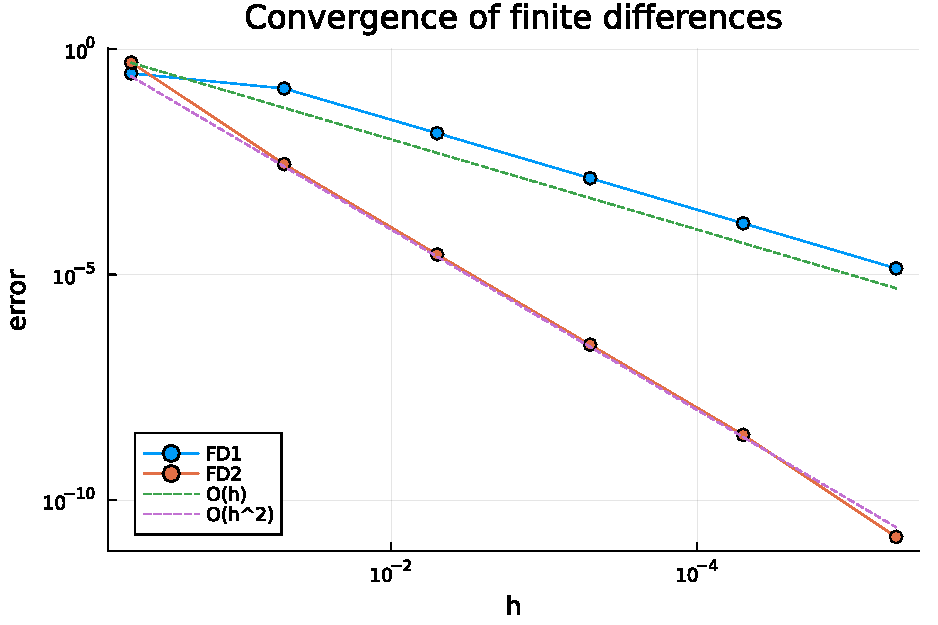
\includegraphics[keepaspectratio]{Lecture14_files/mediabag/Lecture14_files/figure-pdf/cell-13-output-1.pdf}}

\subsection{Stability}\label{stability}

In addition to the truncation error (the planned and understood error),
there is round-off error. Consider the forward difference
\[\delta(h) = \frac{f(x+h) - f(x)}{h}.\]

As \(h \rightarrow 0\), the numerator approaches zero even though the
values involved are not necessarily near 0. This is the recipe for
subtractive cancellation error! In fact, these formulas are inherently
ill-conditioned as \(h \rightarrow 0\).

Recall that the condition number for the problem of computing
\(f(x+h) - f(x)\) is
\[\kappa(h) = \frac{\max\{|f(x+h)|,|f(x)|\}}{|f(x+h)-f(x)|}.\]

\begin{center}\rule{0.5\linewidth}{0.5pt}\end{center}

Hence, the numerical value we actually compute for \(\delta\) is
\[\begin{align*}
\tilde{\delta}(h) &= \frac{f(x+h) - f(x)}{h} (1 + \kappa(h)\epsilon_{\text{mach}})
\\&= \delta(h) + \frac{\max\{|f(x+h)|,|f(x)|\}}{|f(x+h)-f(x)|} \frac{f(x+h) - f(x)}{h} \epsilon_{\text{mach}}
\end{align*}\]

As \(h \rightarrow 0\),
\[|\tilde{\delta}(h) - \delta(h)| = \frac{\max\{|f(x+h)|,|f(x)|\}}{h} \epsilon_{\text{mach}} \sim |f(x)| \epsilon_{\text{mach}} h^{-1}.\]

Combining the truncation and roundoff errors yields
\[|f'(x) - \tilde{\delta}(h)| \le |\tau_f(h)| + |f(x)| \epsilon_{\text{mach}} h^{-1}.\]

As the truncation error decreases as \(h\) decreases, the roundoff error
actually \emph{increases} due to subtractive cancellation.

\begin{center}\rule{0.5\linewidth}{0.5pt}\end{center}

At around \(h \approx K \sqrt{\epsilon_{\text{mach}}}\), these errors
are roughly the same size. For this first-order finite-difference
method, the optimal spacing between nodes is proportional to
\(\sqrt{\epsilon_{\text{mach}}}\).

\begin{tcolorbox}[enhanced jigsaw, left=2mm, arc=.35mm, leftrule=.75mm, colbacktitle=quarto-callout-warning-color!10!white, coltitle=black, toptitle=1mm, bottomtitle=1mm, colback=white, colframe=quarto-callout-warning-color-frame, opacityback=0, breakable, titlerule=0mm, title={Fact:}, rightrule=.15mm, bottomrule=.15mm, toprule=.15mm, opacitybacktitle=0.6]

For computing with a finite-difference method of order \(m\) in the
presence of roundoff, the optimal spacing of nodes satisfies
\[h_{\text{opt}} \approx \epsilon_{\text{mach}}^{1/(m+1)},\] and the
optimal total error is roughly \(\epsilon_{\text{mach}}^{m/(m+1)}\).

\end{tcolorbox}

\begin{Shaded}
\begin{Highlighting}[]
\NormalTok{f }\OperatorTok{=}\NormalTok{ x }\OperatorTok{{-}\textgreater{}} \FunctionTok{exp}\NormalTok{(}\OperatorTok{{-}}\FloatTok{1.3}\OperatorTok{*}\NormalTok{x);}
\NormalTok{exact }\OperatorTok{=} \OperatorTok{{-}}\FloatTok{1.3}

\NormalTok{h }\OperatorTok{=}\NormalTok{ [ }\FloatTok{1}\OperatorTok{/}\FloatTok{10}\OperatorTok{\^{}}\NormalTok{n for n }\KeywordTok{in} \FloatTok{1}\OperatorTok{:}\FloatTok{12}\NormalTok{ ]}
\NormalTok{FD1, FD2, FD4 }\OperatorTok{=}\NormalTok{ [], [], []}
\ControlFlowTok{for}\NormalTok{ h }\KeywordTok{in}\NormalTok{ h }
\NormalTok{    nodes }\OperatorTok{=} \FunctionTok{h*}\NormalTok{(}\OperatorTok{{-}}\FloatTok{2}\OperatorTok{:}\FloatTok{2}\NormalTok{)}
\NormalTok{    vals }\OperatorTok{=}\NormalTok{ @. }\FunctionTok{f}\NormalTok{(nodes)}
    \FunctionTok{push!}\NormalTok{(FD1, }\FunctionTok{dot}\NormalTok{([ }\FloatTok{0} \FloatTok{0} \OperatorTok{{-}}\FloatTok{1} \FloatTok{1} \FloatTok{0}\NormalTok{ ]}\OperatorTok{/}\NormalTok{h,vals))}
    \FunctionTok{push!}\NormalTok{(FD2, }\FunctionTok{dot}\NormalTok{([ }\FloatTok{0} \OperatorTok{{-}}\FloatTok{1}\OperatorTok{/}\FloatTok{2} \FloatTok{0} \FloatTok{1}\OperatorTok{/}\FloatTok{2} \FloatTok{0}\NormalTok{ ]}\OperatorTok{/}\NormalTok{h,vals))}
    \FunctionTok{push!}\NormalTok{(FD4, }\FunctionTok{dot}\NormalTok{([ }\FloatTok{1}\OperatorTok{/}\FloatTok{12} \OperatorTok{{-}}\FloatTok{2}\OperatorTok{/}\FloatTok{3} \FloatTok{0} \FloatTok{2}\OperatorTok{/}\FloatTok{3} \OperatorTok{{-}}\FloatTok{1}\OperatorTok{/}\FloatTok{12}\NormalTok{ ]}\OperatorTok{/}\NormalTok{h, vals))}
\ControlFlowTok{end}

\NormalTok{table }\OperatorTok{=}\NormalTok{ [h FD1 FD2 FD4]}
\FunctionTok{pretty\_table}\NormalTok{(table[}\FloatTok{1}\OperatorTok{:}\FloatTok{4}\NormalTok{,}\OperatorTok{:}\NormalTok{],header}\OperatorTok{=}\NormalTok{[}\StringTok{"h"}\NormalTok{,}\StringTok{"FD1"}\NormalTok{,}\StringTok{"FD2"}\NormalTok{,}\StringTok{"FD4"}\NormalTok{])}
\end{Highlighting}
\end{Shaded}

\begin{verbatim}
┌────────┬──────────┬──────────┬──────────┐
│      h │      FD1 │      FD2 │      FD4 │
├────────┼──────────┼──────────┼──────────┤
│    0.1 │ -1.21905 │ -1.30366 │ -1.29999 │
│   0.01 │ -1.29159 │ -1.30004 │     -1.3 │
│  0.001 │ -1.29916 │     -1.3 │     -1.3 │
│ 0.0001 │ -1.29992 │     -1.3 │     -1.3 │
└────────┴──────────┴──────────┴──────────┘
\end{verbatim}

\begin{center}\rule{0.5\linewidth}{0.5pt}\end{center}

\begin{Shaded}
\begin{Highlighting}[]
\NormalTok{err }\OperatorTok{=}\NormalTok{ @. }\FunctionTok{abs}\NormalTok{([FD1 FD2 FD4] }\OperatorTok{{-}}\NormalTok{ exact)}

\FunctionTok{plot}\NormalTok{(h,err,m}\OperatorTok{=:}\NormalTok{o,label}\OperatorTok{=}\NormalTok{[}\StringTok{"FD1"} \StringTok{"FD2"} \StringTok{"FD4"}\NormalTok{],}
\NormalTok{    xaxis}\OperatorTok{=}\NormalTok{(}\OperatorTok{:}\NormalTok{log10,}\StringTok{"h"}\NormalTok{),xflip}\OperatorTok{=}\ConstantTok{true}\NormalTok{,yaxis}\OperatorTok{=}\NormalTok{(}\OperatorTok{:}\NormalTok{log10,}\StringTok{"error"}\NormalTok{), }
\NormalTok{    title}\OperatorTok{=}\StringTok{"FD error with roundoff"}\NormalTok{,legend}\OperatorTok{=:}\NormalTok{bottomright)}

\FunctionTok{plot!}\NormalTok{(h,}\FloatTok{0.1}\FunctionTok{*eps}\NormalTok{()}\OperatorTok{./}\NormalTok{h,l}\OperatorTok{=:}\NormalTok{dash,color}\OperatorTok{=:}\NormalTok{black,label}\OperatorTok{=}\StringTok{"O(h\^{}\{{-}1\})"}\NormalTok{)}
\end{Highlighting}
\end{Shaded}

\pandocbounded{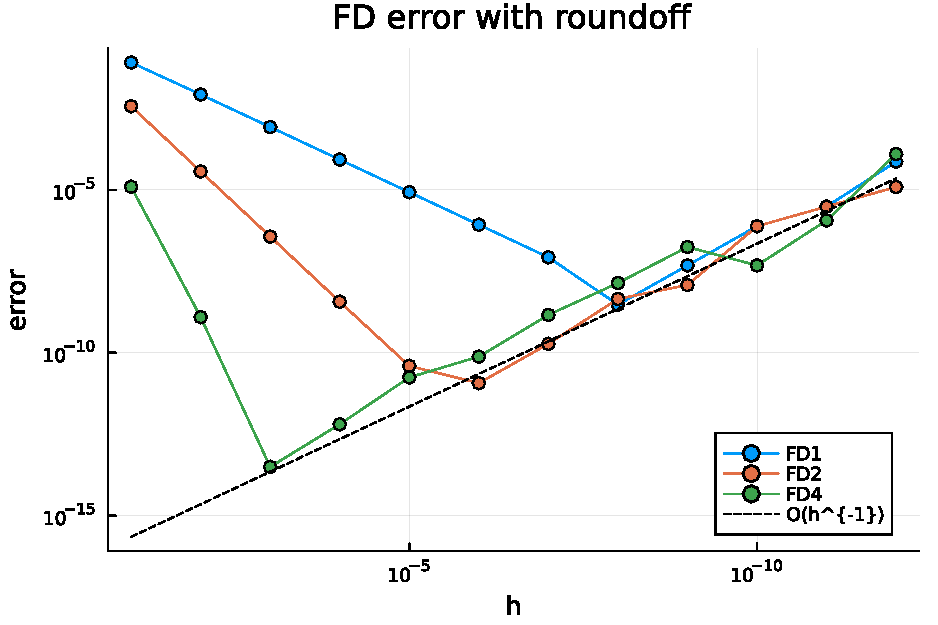
\includegraphics[keepaspectratio]{Lecture14_files/mediabag/Lecture14_files/figure-pdf/cell-15-output-1.pdf}}

The error is initially dominated by truncation error, but eventuallly
the roundoff error dominates.




\end{document}
